\documentclass{article}

\usepackage[T2A]{fontenc}
\usepackage[utf8]{inputenc}
\usepackage[russian]{babel}
\usepackage{MnSymbol,wasysym}
\usepackage[unicode, colorlinks, linkcolor=blue, citecolor=blue]{hyperref}

\usepackage{multirow}
\usepackage{hhline}
\usepackage{graphicx}
\graphicspath{{pictures/}}
\DeclareGraphicsExtensions{.pdf,.png,.jpg}


\usepackage[T2A]{fontenc}
\usepackage[utf8]{inputenc}
\usepackage[russian]{babel}


\usepackage[unicode, colorlinks, linkcolor=blue, citecolor=blue]{hyperref}
\usepackage{amsmath}
\usepackage{graphicx}
\graphicspath{{pictures/}}
\DeclareGraphicsExtensions{.pdf,.png,.jpg}

\usepackage{pgfplots}
\usepackage{tikz}

\usepackage[]{geometry}
\geometry
{
	a4paper,
	total={170mm,257mm},
	left=25mm,
	top=19mm,
	right=25mm
}

\begin{document}
	\selectlanguage{russian}
	%----------------------------------Шапка------------------------------------—
	\begin{figure}[htb]
		\begin{minipage}[c]{0.12\textwidth}
			
\includegraphics[scale=0.25]{AU}
		\end{minipage}
		\hfill
		\begin{minipage}[t]{0.9\textwidth}
			{\Large\bfseries Санкт-Петербургский национальный исследовательский Академический университет имени Ж.И.~Алфёрова\\Российской академии наук}
		\end{minipage}
		\rule{164mm}{0.3mm}
	\end{figure}
	
	\begin{center}
		{\large\textbf{Рабочий протокол и отчёт по лабораторной работе №1 }}\\
		{\large{Александр Слободнюк, Свиридов Федор, Владимир Попов}}
	\end{center}
	\begin{center}
		\Large\bfseries{«Исследование законов механических колебаний с помощью крутильного маятника Поля»}\\
	\end{center}

	
	
	
	
	\paragraph\large{\bf{Цель работы:}}
	Изучить понятие о колебаниях, вращательном движении, свободных и вынужденных колебаниях.
	\paragraph{Задачи, решаемые при выполнении работы:}
	\begin{enumerate}
		\item Начать процесс колебаний маятника, при разных значениях I
		\item Сделать запись экспериментов
		\item Измерить значение амплитуды
	\end{enumerate}
	\paragraph{Объект исследования:}
	Свободные затухающие колебания
	\paragraph{Метод экспериментального исследования}
	\begin{enumerate}
		\item Измерение амплитуды колебаний в разные моменты времени
		\item Измерение периода колебаний
	\end{enumerate}
	\paragraph{Рабочие формулы:}
	\begin{equation}
		\large{\beta}=\frac{-\Sigma_it_i\ln{\frac{\alpha_{cp_i}}{\alpha_0}}}{\Sigma_it_{i}^2}
	\end{equation}
	\begin{equation}
		\large{\omega_0} = \sqrt{(\omega^2+\beta^2)}
	\end{equation}
	\begin{equation}
		\large{\omega} = \frac{2\pi}{T}
	\end{equation}
	
	
	\paragraph{Cхема установки:}
	\begin{center}
		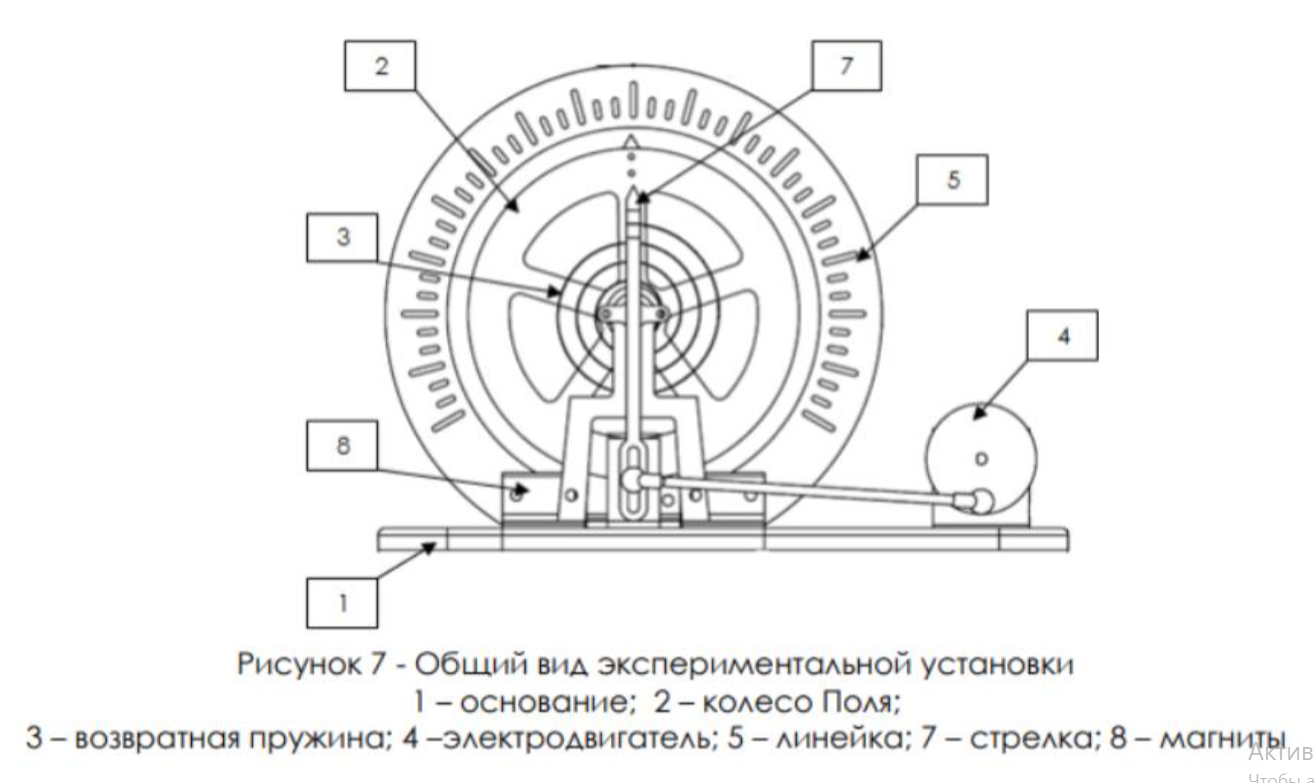
\includegraphics[scale=0.5]{Маятник Поля 2}
	\end{center}
	\paragraph{Результаты прямых измерений и их обработки}
	
	
	\begin{center}
		\textbf{Экспериментальные данные из опыта, проведенного в отсутствии напряжения}
		\begin{tabular}{|c|c|c|c|c|c|c|c|c|c|c|}
			\hline
			t & $\alpha_1 (deg)$ & $\alpha_2 (deg)$ & $\alpha_3 (deg)$ & $\alpha_{cp} (deg)$ & $\alpha_0 (deg)$ & T, c & $\frac{\alpha_{cp}}{\alpha_0}$ & $\log{\frac{\alpha_{cp}}{\alpha_0}}$ & $t\log{\frac{\alpha_{cp}}{\alpha_0}}$ & $t^{2}$ \\
			\hline
			T & 55 & 55 & 54,5 & 54,6 & & & 0.908 & -0,096 & -0,096 & 1 \\
			\hhline{-----~~----}
			2T & 50 & 49 & 49 & 49,5 & & & 0,82 & -0,2 & -0,4 & 4 \\
			\hhline{-----~~----}
			3T & 45 & 44 & 44 & 44,6 & 60 & 1 & 0,743 & -0,3 & -0,9 & 9 \\
			\hhline{-----~~----}
			4T & 40 & 40 & 39,5 & 39,8 & & & 0,663 & -0,41 & -1,6 & 16 \\
			\hhline{-----~~----}
			5T & 35 & 35 & 35 & 35 & & & 0,583 & -0,54 & -2,7 & 25 \\
			\hline
		\end{tabular}
	\end{center}
	
	\begin{center}
		\textbf{Экспериментальные данные, полученные при I = 4A}
		\begin{tabular}{|c|c|c|c|c|c|c|c|c|c|c|}
			\hline
			t & $\alpha_1 (deg)$ & $\alpha_2 (deg)$ & $\alpha_3 (deg)$ & $\alpha_{cp} (deg)$ & $\alpha_0 (deg)$ & T, c & $\frac{\alpha_{cp}}{\alpha_0}$ & $\log{\frac{\alpha_{cp}}{\alpha_0}}$ & $t\log{\frac{\alpha_{cp}}{\alpha_0}}$ & $t^{2}$ \\
			\hline
			T & 54,5 & 50 & 58 & 54,2 & & & 0.9 & -0,1 & -0,096 & 1 \\
			
			\hhline{-----~~----}
			2T & 52,5 & 45 &52,5 & 50 & & & 0,83 & -0,18 & -0,36 & 4 \\
			\hhline{-----~~----}
			3T & 47 & 40 & 51 & 47,6 & 60 & 1 & 0,80 & -0,23 & -0,69 & 9 \\
			\hhline{-----~~----}
			4T & 42,5 & 35 & 46 & 41,2 & & & 0,69 & -0,38 & -1,5 & 16 \\
			\hhline{-----~~----}
			5T & 37,5 & 30 & 41 & 36,2 & & & 0,603 & -0,50 & -2,5 & 25 \\
			\hline
		\end{tabular}
		
	\end{center}
	
	\begin{center}
		\textbf{Экспериментальные данные, полученные при I = 5A}
		\begin{tabular}{|c|c|c|c|c|c|c|c|c|c|c|}
			\hline
			t & $\alpha_1 (deg)$ & $\alpha_2 (deg)$ & $\alpha_3 (deg)$ & $\alpha_{cp} (deg)$ & $\alpha_0 (deg)$ & T, c & $\frac{\alpha_{cp}}{\alpha_0}$ & $\log{\frac{\alpha_{cp}}{\alpha_0}}$ & $t\log{\frac{\alpha_{cp}}{\alpha_0}}$ & $t^{2}$ \\
			\hline
			T & 55 & 54,5 & 51 & 53,5 & & & 0.9 & -0,12 & -0,12 & 1 \\
			\hhline{-----~~----}
			2T & 49 & 47 & 44 & 45 & & & 0,75 & -0,29 & -0,58 & 4 \\
			\hhline{-----~~----}
			3T & 43 & 41 & 37,5 & 40,5 & 60 & 1 & 0,675 & -0,4 & -1,8 & 9 \\
			\hhline{-----~~----}
			4T & 36 & 36 & 32 & 34,7 & & & 0,57 & -0,55 & -2,2 & 16 \\
			\hhline{-----~~----}
			5T & 31 & 31 & 25,5 & 29,2 & & & 0,49 & -0,72 & -3,6 & 25 \\
			\hline
		\end{tabular}
	\end{center}
	
	
	\paragraph{Проведенные расчеты:}
	 Во всех опытах значение $\omega$ равно $2\pi$, так как период колебаний T во всех экспериментах был равен одной секунде
	
	
		$$\large{\beta_1}=\frac{-\ln{\frac{54,6}{60}}-2\ln{\frac{49,5}{60}}-3\ln{\frac{44,6}{60}}-4\ln{\frac{39,8}{60}}-5\ln{\frac{35}{60}}}{1+4+9+16+25}\approx0,103$$
	
	
		$$\large{\beta_2}=\frac{-\ln{\frac{54,2}{60}}-2\ln{\frac{50}{60}}-3\ln{\frac{47,6}{60}}-4\ln{\frac{41,2}{60}}-5\ln{\frac{36,2}{60}}}{1+4+9+16+25}\approx0,0938$$
	
	$$	\large{\beta_3}=\frac{-\ln{\frac{53,5}{60}}-2\ln{\frac{45}{60}}-3\ln{\frac{40,5}{60}}-4\ln{\frac{34,7}{60}}-5\ln{\frac{29,2}{60}}}{1+4+9+16+25}\approx0,139$$

	$$	\large{\omega_1}= \sqrt{6,283^2+0,106^2} \approx6,2839$$

	$$	\large{\omega_2}= \sqrt{6,283^2+0,0938^2} \approx6,2837$$

	$$	\large{\omega_3}= \sqrt{6,283^2+0,139^2} \approx6,2845$$

	$$	\large{\omega}= 2\pi$$
 
\paragraph{Погрешности:} $\ast$
$$\Delta_i\ln{\frac{\alpha_{cp_i}}{\alpha_{0}}} \approx \frac{\Delta\alpha_{cp_i}}{\alpha_{cp_i}} $$
$$A = max(\Delta_i\ln{\frac{\alpha_{cp_i}}{\alpha_{0}}}) $$

$$\Delta\beta \approx \frac{A + 2A +3A
	+4A +5A}{1 + 4 + 9 + 16 +25}$$
$$\Delta\beta_1 \approx0,05$$
$$\Delta\beta_2 \approx0,05$$
$$\Delta\beta_3 \approx0,06$$

$$ \Delta\omega_0 = \frac{\beta\Delta\beta}{\sqrt{\omega^2 + \beta^2}}$$
$$\Delta\omega_0\approx0,001$$
	\paragraph{Графические изображения зависимости амплитуды от времени:}
	\begin{center}
		\begin{tikzpicture}
			\begin{axis}[title = {Зависимость амплитуды от времени без напряжения }, xlabel={$T,c$}, ylabel={$\alpha, deg$}]
				\addplot coordinates{(0,60) (1,54.6) (2,49.5) (3,44.6) (4,39.8) (5,35)};
			\end{axis}
		\end{tikzpicture}
	\end{center}
	
	\begin{center}
		\begin{tikzpicture}
			\begin{axis}[title={Зависимость амплитуды от времени при I = 4А}, xlabel={$T,c$}, ylabel={$\alpha, deg$}]
				\addplot[orange] coordinates{(0,60) (1,54.2) (2,50) (3,47.6) (4,41.2) (5,36.2)};
			\end{axis}
		\end{tikzpicture}
	\end{center}
	
	\begin{center}
		\begin{tikzpicture}
			\begin{axis}[title={Зависимость амплитуды от времени при I = 5А}, xlabel={$T,c$}, ylabel={$\alpha, deg$}]
				\addplot[pink] coordinates{(0,60) (1,53.5) (2,45) (3,40.5) (4,34.7) (5,29.2)};
			\end{axis}
		\end{tikzpicture}
	\end{center}
	
	\paragraph{Окончательные результаты}
	\begin{enumerate}
		\item $\large{\beta_1}\approx0,10\pm0,05$
		\item $\large{\beta_2}\approx0,09\pm0,05$
		\item $\large{\beta_3}\approx0,14 \pm0,06$
		\item $\large{\omega_1} \approx(6,284\pm0,001)\;\mbox{Гц}$
		\item $\large{\omega_2} \approx(6,284\pm0,001)\;\mbox{Гц}$
		\item $\large{\omega_3} \approx(6,285\pm0,001)\;\mbox{Гц}$
	\end{enumerate}
	
	\paragraph{Вывод:}
	Мы провели несколько экспериментов, в которых измеряли значения амплитуды колебаний в разные моменты времени. На основе полученных данных мы провели расчеты и нашли значения коэффициента затухания и собственной частоты колебаний системы. Эти величины должны быть тем больше, чем больше сила сопротивления (в наших опытах она регулировалась изменением силы тока, прямо прапорциональной этой силе). На самом деле получилось так, что коэффициенты затухания хоть сколько-то заметно отличаются между собой, в то время как частоты колебаний практически
	
	одинаковы. К тому же не имеет место монотонность этих значений: во втором эксперименте коэффициент затуханий, а вместе с ним и собственная частота системы меньше, чем в первом опыте. Такой результат может быть объяснен тем, что в этой работе вычисления очень чувствительны к неточным измерениям - логарифм от двух разных на очень небольшую величину чисел меньших единицы заметно отличается по значению. Почти полное совпадение $\omega_1, \omega_2$ и $\omega_3$ произошло из-за того, что сила сопротивления была не слишком большой; амплитуда экспоненциально убывает с увеличением силы, в то время как $\omega_0$ по формуле 2 увеличивается как корень из суммы квадратов частоты колебаний и коэффициента затухания, который почти не вносит вклад в вычисления, если он по порядку меньше единицы.
\end{document}